\documentclass[tikz, border=2mm]{standalone}
\usetikzlibrary{positioning, matrix, arrows.meta,calc}

\begin{document}
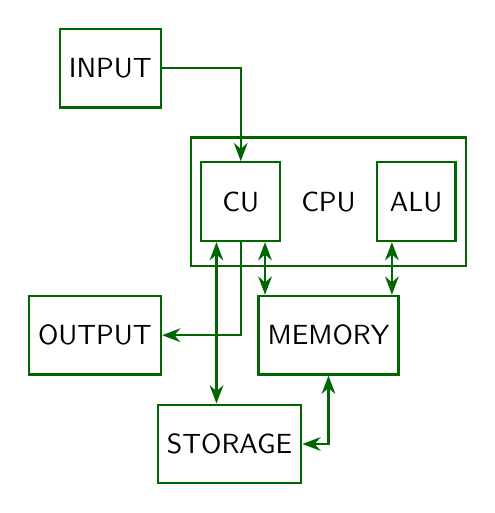
\begin{tikzpicture}[
    myline/.style={draw=green!40!black, thick},
    box/.style={myline, minimum height=1cm, minimum width=1cm, font=\sffamily, inner sep=.3333em}, >=Stealth]

    \matrix (CPU) [matrix of nodes, inner ysep=3mm, nodes=box, myline, column sep=1mm]
        {|(CU)|CU & |[draw=none]|CPU & |(ALU)| ALU \\};
    \node[box, above left=5mm of CPU] (input) {INPUT};

    \node[box, below left=5mm of CPU] (output) {OUTPUT};
    \node[box, at=(CPU|-output)] (memory) {MEMORY};
    \node[box, below left=5mm of memory, anchor=north] (storage) {STORAGE};

    \draw[<->, myline] (storage)-|(memory);
    \draw[->,myline] (input)-|(CU);
    \draw[->,myline] (CU)|-(output);

    \draw[<->, myline] ($(CU.south west)!.2!(CU.south east)$) coordinate (aux)--(aux|-storage.north);
    \draw[<->, myline] ($(CU.south west)!.8!(CU.south east)$) coordinate (aux)--(aux|-memory.north);
    \draw[<->, myline] ($(ALU.south west)!.2!(ALU.south east)$) coordinate (aux)--(aux|-memory.north);
\end{tikzpicture}
\end{document}
